\chapter{Proposta deste projeto}

Este capítulo traz uma breve descrição das características intrínsecas a um \textit{framework}, seguida por uma definição das principais características que determinam a sua natureza, consideradas determinantes para o desenvolvimento deste trabalho. em seguida é apresentada algumas soluções existentes para o desenvolvimento de simulações distribuídas de eventos discretos e por fim é apresentado o modelo desenvolvido neste trabalho, tanto como suas principais características e diferenciações em relação às soluções atualmente existentes.

\section{Um \textit{framework} para simulação distribuída}

Escrever uma aplicação de simulação de eventos discretos distribuída é uma tarefa de grandes proporções. Todo o tratamento de sincronização, comunicação, troca de mensagens, manipulação de objetos remotos, entre outras tarefas, acarretam no surgimento de diversas detalhes, alheios à simulação propriamente dita, que devem ser gerenciadas pelo desenvolvedor que pretende implementar a simulação.

Somam-se a isso questões de ordem prática, como cuidado com o desempenho (entram neste ítem balanceamento de carga, \textit{design} eficiente dos algorítmos utilizados, etc) e permissividade ao erro (a probabilidade de se intruduzir um erro em um código aumente proporcionalmente ao tamanho deste código, \cite{HONGYU09}) e obtem-se neste ponto um cenário onde o desenvolvedor acaba tendo que se preocupar demasiadamente com detalhes alheios à simulação, tornando a simulação uma tarefa dispendiosa e altamente propensa a erros.

Assim como proposto em \cite{LIVERSON}, um framework de simulação tem o objetivo de suportar o desenvolvimento de simulações distribuídas de uma maneira que proveja encapsulamento dos mecanismos alheios à modelagem e execução da simulação, transparência nas tomadas de decisões internas e reusabilidade de código.

A opção por um \textit{framework} acarreta em uma série de vantagens por excluir de seu usuário a responsabilidade de gerenciar diversas tarefas internas, deixando-o focado apenas na criação do modelo a ser simulado. Para prover tal separação entre a aplicação escrita pelo usuário e o \textit{framework}, este compromete-se a prover três funcionalidades essenciais: encapsulamento, transparência e reusabilidade.

\subsection{Encapsulamento}

Uma das funções de um \textit{framework} é encapsular diversos elementos que não tratam diretamente da simulação, porém sustentam funcionalidades que dão vida a esta. Exemplo disso é a possibilidade de se isolar elementos lógicos para representar o modelo a ser simulado. Quando encapsulamos o funcionamento de uma fila de eventos ou o de um processo lógico em uma classe, por exemplo, estamos isolando sua implementação e seus detalhes do usuário final do \textit{framework}. Ao usuário cabe reutilizar estes componentes e, quando julgar necessário, criar componentes baseados nesses primitivos.

Outros exemplos de ocasiões em que se pode aplicar o encapsulamento é tanto nos algorítmos responsáveis pelo balanceamento de cargas no sisteam quanto nos mecanismos de sincronização de processos lógicos. A possibilidade de encapsular esses componentes do \textit{framework} em classes separadas nos possibilita o intercâmbio de diferentes implementações que solucionam um mesmo problema. Com uma interface bem desenvolvida, pode se criar, por exemplo, encapsulamentos distintos para o protocolo \textit{Time Warp} e para o protocolo \textit{Rollback} Solidário. Isso permitiria que o usuário escolhesse, antes de iniciar a simulação, qual protocolo pretende adotar no processo.

\subsection{Transparência}

A proposta de se escrever um código que seja ao mesmo tempo fácil de se implementar pelo usuário do \textit{framework} e eficiente em sua execução projeta-se diretamente na utilização de diversas camadas que ao mesmo tempo esconde do usuário do \textit{framework} algumas decisões internas e provê abstrações nas quais o usuário se apóia para desenvolver seu modelo.

Segundo \cite{DIRK00}, um usuário ao utilizar um \textit{framework} reutiliza seu \textit{design} e sua implementação. Isto é feito pois cabe ao framework resolver os problemas referentes ao seu domínio (no caso proposto por esse trabalho: sincronização, comunicação, migração e balanceamento de carga em um sistema distribuído de simulação de eventos discretos), deixando ao usuário apenas a função de desenvolver o modelo, sem a necessidade de se preocupar com questões que estão fora de seu domínio.

O conceito de transparência neste caso remete-se na intenção do \textit{framework} que é deixar invisível ao seu usuário toda e qualquer decisão que não compete à construção do seu modelo a ser simulado. Isso acaba trazendo para a construção do \textit{framework} algumas responsabilidades quanto a tomadas de decisões sobre \textit{design} de software, implementação de algorítmos considerados decisivos, entre outras.

\subsection{Reusabilidade}

Ao se eleborar um \textit{framework}, o responsável pelo seu \textit{design} deve permitir que componentes internos deste sejam trocados ou mesmo customizados. Isso garante que que o mesmo código escrito para ser executando em um determinado \textit{framework} continue a funcionar mesmo depois da troca de algum componente interno deste \textit{framework}.

No caso da simulação distribuída, componentes como os protocolos de sincronização ou o sistema de balanceamento de cargas poderiam ser plugáveis. Isto permitiria customizar o comportamento do \textit{framework} apenas selecionando estes componentes, o que permitiria que simulássemos o mesmo modelo (sem alterações) usando diferente soluções para sincronização, balanceamento de carga, etc. Esta flexibilidade garante a reutilização de código, economizando no desenvolvimento da simulação e dinamizando a comparação entre diferentes soluções para um mesmo modelo.

\section{Soluções Existentes \label{solucoes_existentes}}

Uma proposta de \textit{framework} para simulação distribuída foi apresentada por \cite{LIVERSON}, baseada em troca de mensagens suportando tanto \textit{MPI} quanto \textit{PVM} e abordando tanto os protocolos de sincronização \textit{Rollback} Solidário e \textit{Time Warp}. Em \cite{RIBEIROALVES} é proposto uma solução utilizando agentes móveis, o que contempla, além da comunicação por troca de mensagens, também a possibilidade de migrações de processos lógicos através dos nós do sistema distribuído, visando a possibilidade de balancear as cargas no sistema.

Algumas propostas como a \textit{Remote Call Framework (RCF)}, \textit{ClassdescMP} e diversas implementações do \textit{MPI} e de \textit{PVM} provém soluções para a a troca de mensagem entre diferentes processos. Essas soluções provém eficientes mecanismos para gerenciar a troca de mensagens, porém não possuem soluções nativas para a migração de processos lógicos entre nós do sistema de simulação, e também não estão preparados para o redirecionamento de mensagens enviadas à processos que migraram para um nó diferente do seu nó de origem.

Outras soluções como \cite{SASSY} e \cite{}, assim como \cite{RIBEIROALVES}, baseiam-se nos agentes móveis para se desenvolver a aplicação de simulação distribuída. As soluções baseadas em agentes móveis proporcionama uma mobilidade aos processos lógicos, útil ao balanceamento de carga. Porém, assim como as bibliotecas de comunicação citadas anteriormente, não estão preparadas para redirecionar as mensagens destinadas à processos que migraram de seus nós de origem.

Visando isso este trabalho propõe apresentar uma solução, em formato de \textit{fremowork}, para o desenvolvimento de simulações distribuídas de eventos discretos. Este \textit{framework} deve possibilitar ao seu usuário descrever o modelo a ser simulado de forma simples, e simulá-lo em diferentes configurações (diferentes protocolos de sincronizaçao, de forma centralizada ou distribuída, etc) apenas modificando suas configurações, sem a necessidade de alterar o código que descreve o modelo a ser simulado.

Para que sejam sustentados tanto os mecanismos de sincronização da simulação quanto o balanceamento de cargas, é vital que o \textit{framework} supra, internamente, as necessidades básicas de comunicação, troca de mensagens, migração de processos lógicos e comunicação grupal entre os processos. Estas funcionalidades são providas pelo \textit{middleware} de comunicação do \textit{framework}. 

Uma característica fundamental do \textit{middleware} de comunicação proposto por esse trabalho é que, uma vez um objeto migrando de seu nó de origem para um novo local, o \textit{middleware} se encarrega de redirecionar as mensagens destinadas à esse processo lógico em seu novo ambiente, deixando completamente transparente para o usuário questões como endereço físico do processo lógico, \textit{status} do processo, etc.

\section{Arquitetura proposta}

A figura~\ref{fig:arquitetura_macro} apresenta uma visão ampla da arquitetura do framework de simulação distribuída aqui proposto.

A camada superior, denominada aplicação, é a interface pela qual o usuário do sistema descreve o seu modelo a ser simulado. Cabe ao \textit{framework} prover uma \textit{API} com a qual o usuário descreverá o comportamento do seu modelo.

A camada intermediária compreende tanto os algorítmos responsáveis pelo gerenciamento da simulação (o \textit{kernel} do \textit{framework}) quanto os mecanismos de sincronização e balanceamento de carga. É nesta camada também que se encontra as descrições dos componentes elementares utilizados para a descrição do modelo. São exemplos de componentes: fila de eventos futuros, gerador de eventos e o processo lógico, responsável por consumir os eventos discretos.

Por fim, sustentando as demais camadas encontra-se o \textit{middleware} de comunicação. Esta camada é responsável não somente pela troca de mensagens entre processos lógicos, como também por todo o gerenciamento do ciclo de vida de um processo, serialização e migração de processos lógicos, redirecionamento de mensagens, gerenciamento de recursos do sistema e mecanismo de comunicação grupal. 

\begin{figure}
  \centerline{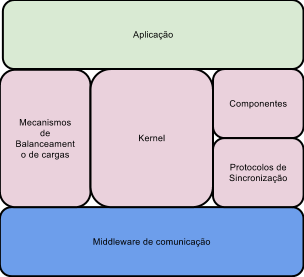
\includegraphics{arquitetura_macro.png}}
  \caption{Camadas da arquitetura do \textit{framework}.}
\label{fig:arquitetura_macro}
\end{figure}

Conforme descrito na seção~\ref{solucoes_existentes}, os mecanismos de troca de mensagens existentes não possuem uma camada de abstração do endereço de um componente após uma eventual migração. Isto significa que ao se migrar um componente de seu nó de horigem para um novo ambiente tenhamos que, de maneira explícitar, avisar a todos os componentes do sistema que o seu endereço físico mudou, para que as mensagens direcionadas a este processo lógico o alcancem em seu novo ambiente de execução.

Nos casos que mais se aproximam deste requesito do sistema, os agentes móveis, há uma transparência na troca de mensagens até o momento em que um agente migra para um diferente nó no sistema. Ao se mover para um ambiente diferente do seu ambiente de origem, implementações de agentes móveis como \textit{Aglets} requerem uma intervenção do usuário para que se refatore os valores dos endereços físicos dos objetos para que se possa continuar a somunicação. O middleware aqui proposto visa resolver este problema, tornando a comunicação entre processos completamente transparente para o seu usuário, mesmo após a migração de uma componente de seu nó de origem.

\section{Organização deste documento}

Os capítulos seguintes tratam da descrição detalhada da arquitetura do projeto e de sua implementação. O capítulo quatro trata da arquitetura do \textit{middleware} de comunicação. O capítulo cinco traz detalhes da arquitetura do \textit{framework} de simulação.

No capítulo seis é demonstrado detalhes de implementação que o autor julga conveniente descrever neste documento e alguns exemplos de simulação utilizando o framework desenvolvido.

Por fim o capítulo sete traz as discussões sobre os resultados desse trabalho, tanto quanto conclusões e propostas para sua continuaidade em trabalhos futuros.
